\documentclass[a4paper]{article}

\usepackage{geometry}
\usepackage[francais]{babel}
\usepackage[utf8]{inputenc}
\usepackage{graphicx}
\usepackage[T1]{fontenc}
\usepackage{listings}
\usepackage{caption}
\usepackage{subcaption}

\title{Projet de Machine Learning - Spaceship Titanic}
\author{Antoine ROUMILHAC \\ Alban RIO \\ Nabil DJELLOUDI \\ Mohammed Yacine BRAHMIA}
\date{Mars 2024}

\newcommand{\illustration}[3]{
    \begin{figure}[h!]
        \centering
        \includegraphics[width=#3]{#1}
        \caption{#2}
    \end{figure}
}

\begin{document}
    \maketitle

    Nom de l'équipe Kaggle : On coule

    \section{Analyse des données}

    \subsection{Répartition passagers transportés / non transportés}

    Dans les données d'entraînement, 4378 des passagers ont été transportés, contre 4315 qui ne l'ont pas été, donc l'ensemble est équilibré. On n'aura donc pas à ajouter de poids lors de la phase d'entraînement.

    \subsection{Valeurs manquantes}

    
    Sur la Figure 1, on peut observer qu'il y a des données manquantes dans l'ensemble d'entraînement, mais qu'elles sont globalement réparties entre les différents passagers.
    On va donc pouvoir remplir les données manquantes en exploitant les relations entre les données.
    
    \illustration{images/Figure 1.png}{Heatmap des données manquantes sur l'ensemble d'entraînement}{6cm}
    \subsection{Variables intéressantes}

    La variable CryoSleep semble être très intéressante à utiliser, car comme présenté sur la figure 2, les personnes ayant pris le CryoSleep n'ont très majoritairement pas été transportées,
    et inversement les personnes ayant pris le CryoSleep ont très majoritairement été transportées.
    
    On peut voir sur la figure 3 que les personnes ayant entre 0 et 12 ans ont été transportées en majorité, 
    tandis que celles ayant entre 18 et 25 ans, et entre 30 et 40 ans, ont été peu moins transportées que la moyenne.
    Il serait donc intéressant d'extraire ces tranches d'âge pour les utiliser pour l'entraînement.
    \illustration{images/Figure 2.png}{Répartition des personnes selon le cryosleep et leur état de transport}{6cm}

    
    La figure 4 montre que la majorité des personnes venant de la planète Europa ont été transportés,
    tandis que la majorité des Terriens n'ont pas été transportés. Il serait donc intéressant d'avoir des
    variables booléennes sécifiant si la personne vient d'Europe, ou de Terre.
    
    \illustration{images/Figure 3.png}{Répartition des personnes selon leur âge et leur état de transport}{6cm}
    
    \illustration{images/Figure 4.png}{Répartition des personnes selon leur planète et leur état de transport}{6cm}
    
    Sur la figure 5, on observe une légère tendance selon la destination des passagers.
    Ceux allant à TRAPPIST-1e ont été majoritairement non transportés, tandis que ceux dont la destination est 55 Cancri e
    ont été majoritairement plus transportés. Idem que pour la planète de départ, il faudrait créer une variable booléenne
    qui est à Vrai si le passager va TRAPPIST-1e, et une autre à Vrai si la personne va à 55 Cancri e.

    \illustration{images/Figure 5.png}{Répartition des personnes selon leur destination et leur état de transport}{6cm}
    
    La figure 6 présente les dépenses des passagers dans le Room Service (en échelle logarithmique sur l'axe des abscisses).
    On peut y voir que ceux n'ayant pas dépensé dans le Room Service ont été très majoritairement transportés.
    A l'inverse, parmi la petite part de passagers ayant dépénsé de l'argent, la majorité n'a pas été transportée.
    La tendance est la même pour les autres postes de dépense.
    Il serait donc intéressant d'avoir une variable booléenne à Vrai si le passager a dépensé de l'argent,
    en complément des variables flottantes de dépenses.

    \illustration{images/Figure 6.png}{Répartition des personnes selon leurs dépenses dans le room service et leur état de transport}{6cm}

    Pour analyser les tendances pour l'identifiant des cabines, on l'a découpé selon les indications du sujet :
    le pont (Deck : de A à G et T), le numéro de cabine, et le côté (Side : S ou P)

    On peut observer que les passagers sur les ponts B et C ont été majoritairement transportés,
    tandis que les passagers sur les ponts F et E ont été majoritairement non transportés.
    Aussi, les passagers sur le côté S ont été majoritairement non transportés.
    Il serait donc intéressant de transformer ces deux variables en des variables booléennes
    à Vrai si la cabine du passager se trouve sur le pont B, C, F ou E, et si elle se trouve sur le côté S.

    Concernant le numéro de cabine, on peut observer qu'il y a des intervalles de numéros de cabine, dans lesquels 
    les occupants sont soit majoritairement transportés, soit majoritairement non transportés.
    Il serait donc judicieux de transformer cette distribution d'entiers en un ensemble de variables booléennes,
    reflétant dans quel intervalle le numéro de la cabine du passager se trouve.

    \begin{figure}
        \centering
        \begin{subfigure}{.5\textwidth}
            \centering
            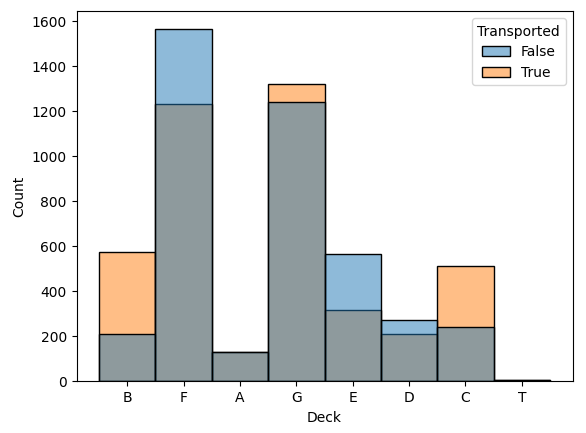
\includegraphics[width=\linewidth]{images/Figure 7.png}
            \caption{Pont (Deck)}
        \end{subfigure}%
        \begin{subfigure}{.5\textwidth}
            \centering
            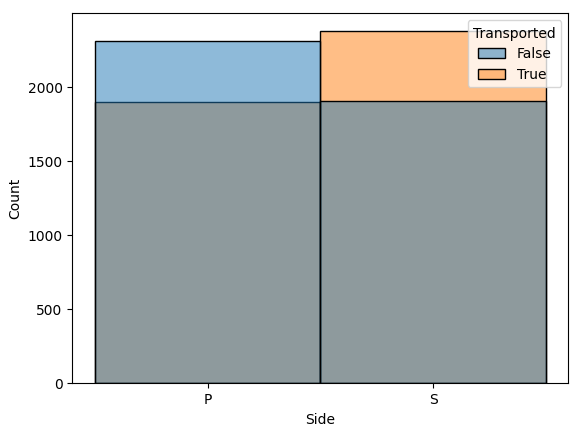
\includegraphics[width=\linewidth]{images/Figure 8.png}
            \caption{Côté (Side)}
        \end{subfigure}
        \begin{subfigure}{.5\textwidth}
            \centering
            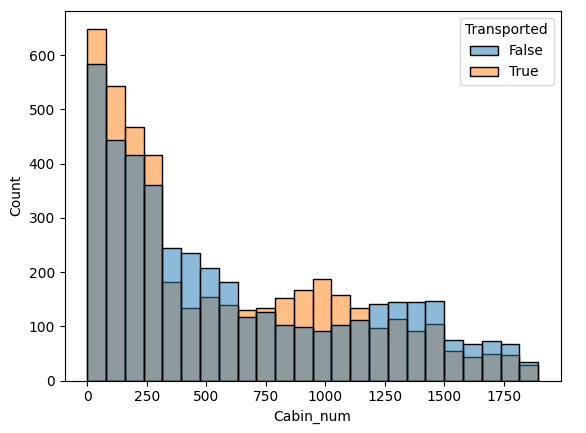
\includegraphics[width=\linewidth]{images/Figure 9.png}
            \caption{Numéro de cabine}
        \end{subfigure}
        \caption{Répartition des passagers selon leur cabine}
    \end{figure}

    \section{Prétraitement des données}

    Avant toute chose, on récupère le numéro de groupe de chaque passager, qui est donné par les 4 premiers chiffres
    de l'identifiant de passager (de la forme GGGG\_NN).

    \subsection{Traitement des données manquantes}

    Comme relevé plus haut, il y a de nombreuses données manquantes dans l'ensemble d'entraînement,
    et elles sont réparties entre un grand nombre de passagers différents, ce qui exclut l'élimination
    des lignes avec des valeurs manquantes.

    On doit donc trouver des relations entre les différentes données disponibles.

    Tous les membres d'un même groupe viennent de la même planète. Donc pour les passagers dont la planète d'origine
    est inconnue et dont au moins un autre passager du même groupe a sa planète d'origine connue,
    on peut en déduire la planète d'origine du passager.

    Pour les passagers dont la cabine est manquante, on fait l'hypothèse qu'ils partagent la même cabine qu'un autre
    membre de leur groupe (arbitrairement, le premier membre qu'on trouve dont la cabine n'est pas inconnue).

    Les personnes en CryoSleep ne dépensent pas d'argent (logique), donc on peut supposer que les personnes
    n'ayant pas dépensé d'argent et dont le statut de CryoSleep est inconnu, sont en CryoSleep.

    Pour les passagers qui ne sont pas en CryoSleep et qui n'ont rien dépensé, on peut raisonnablement supposer que ce sont des enfants
    de moins de 12 ans, car aucun d'entre eux n'a dépensé d'argent dans l'ensemble d'entraînement.

    Les passagers ayant toujours un statut de CryoSleep inconnu voient leur variable CryoSleep mise à Faux,
    étant donné que les passagers étant en CryoSleep sont minoritaires sur le vaisseau.

    Idem concernant les VIP, ceux-ci étant très minoritaires dans le vaisseau, on définit la variable VIP lorsqu'elle est manquante à Faux.

    Pour remplir les valeurs manquantes de pont, on utilise le fait que les Terriens sont majoritairement au pont G,
    tandis que les passagers d'Europa sont majoritairement aux ponts B et C (on utilise leur dépense pour trancher, ceux du deck C étant moins dépensiers).
    Les Martiens sont eux majoritairement sur le pont F.

    A l'inverse, pour finir de remplir les valeurs manquantes des planètes d'origine, on utilise le pont sur lequel sont les passagers.
    Les passagers sur les ponts A, B, C et T sont majoritairement d'Europa, ceux sur E, F et G sont majoritairement des Terriens, tandis que
    ceux sur le pont D sont majoritairement des Martiens.

    Pour finir de remplir les planètes d'origine, on utilise la destination des passagers.
    Ceux allant vers TRAPPIST-1e et PSO J318.5-22 sont en effet en grande partie des Terriens.
    Finalement, pour ceux dont la valeur est encore manquante, on les définit comme venant d'Europa,
    étant donné qu'il y a plus de personnes d'Europa que de Martiens.

    Enfin on définit les destinations manquantes comme étant TRAPPIST-1e, et les âges comme étant l'âge médian.

    Au terme de ces remplissages, nous n'avons donc plus de valeurs manquantes dans l'ensemble.

    \subsection{Choix des variables}

    Tout d'abord, on peut d'ores et déjà éliminer les variables

    \section{Méthodes et paramètres}

    (4) RandomForestClassifier, (3) GradientBoostingClassifier, (2) LGBMClassifier, (5) SVM, (6) GaussianNB, (1) Catboost
    
    Après avoir essayé différents algorithmes de machine learning, nous avons choisi l'algorithme catboost du fait des résultats supérieurs.
    Afin de déterminer les meilleurs paramètres du modèle, nous avons utilisé l'outil RandomizedSearchCV permettant d'essayer un grand nombre 
    de paramètres puis de garder ceux offrant les meilleures performances

    \section{Plan de test}

    \section{Résultats}

    \section{Performances Kaggle}

    Nous avons obtenu un score de 0.81248 ce qui nous met à la 88ème place du classement (au 18 mars 2024).


\end{document}